% vim: set tw=0:
\documentclass{beamer}
\usepackage{graphicx}
%\usepackage{hyperref}
%\hypersetup{pdfborder={0 0 0 0}}

% Reasonable themes:
% Antibes Bergen Berkeley Berlin Frankfurt Goettingen Ilmenau Luebeck Malmoe
% Montpellier PaloAlto Rochester Singapore Szeged Warsaw bars boxes
% compatibility default lined plain shadow sidebar split tree
% And these ones include the author's name on every slide:
% Berkeley

% Declare themes.
\mode<presentation>
\usetheme{UWHEP}

% Personal macros.
\newcommand{\email}[1]{{\texttt #1}}
\newcommand{\newframe}[1]{\section{#1}
    \frametitle{\sc{#1}}}
\newcommand{\subframe}[1]{\subsection{#1}
    \frametitle{\sc{#1}}}
\newcommand{\supers}[1]{\ensuremath{^\textrm{#1}}}
\newcommand{\subs}[1]{\ensuremath{_\textrm{#1}}}
\newcommand{\ca}{\ensuremath{\sim}}

% Author information.
\title{T2 Status}
\author[Maier, Mohapatra]{
    Will Maier \and Ajit Mohapatra\\ 
    {\tt wcmaier@hep.wisc.edu}\\
    {\tt ajit@hep.wisc.edu}}
\institute[Wisconsin]{University of Wisconsin - High Energy Physics}
\date{2008.02.17}
\logo{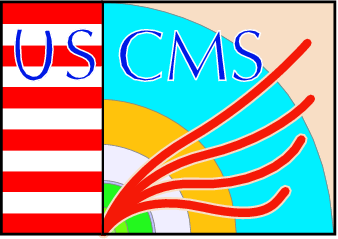
\includegraphics[height=0.6cm]{../../../Graphics/USCMS_logo.png}\hspace{.1cm}
\includegraphics[height=0.75cm]{../../../Graphics/UW_logo.png}}

\begin{document}

\begin{frame}
    \titlepage
\end{frame}

%\section{Overview}
%\begin{frame}
%    \tableofcontents
%\end{frame}

\section{Facilities}
\subsection{Software and Storage}
\begin{frame}
\frametitle{}
\begin{itemize}
    \item Preparing SL5 upgrade
    \item OpenAFS versions $<=$ 1.4.6 eat up lots of the kernel's slab cache
    \begin{itemize}
        \item Will upgrade clients as part of SL5 upgrade
    \end{itemize}
    \item CMSSW\_2\_2\_4 install briefly blocked due to AFS problems
    \item dCache pool RAID suffered simultaneous three disk failure, lost \ca{}400 files
    \begin{itemize}
        \item Backplane/controller appear to be bad, RMAed to vendor
    \end{itemize}
    \item Resolved transfer issues to UCSD [sr107079] and FNAL [sr107123]
    \item Debugged timeouts during collection of dynamic dCache GIP info [sr106989]
    \begin{itemize}
        \item Broke propagation of SE information to BDII, WLCG
        \item \ldots{}which then broke the SAM tests
    \end{itemize}
    \item Killed odd pacman installation jobs submitted by OSG VO user
    \begin{itemize}
        \item Installing from cache at {\tt www.ci.uchicago.edu}
        \item Hangs, causing heavy load on the gatekeeper
    \end{itemize}
\end{itemize}
\end{frame}

\subsection{Production and Monitoring}
\begin{frame}
\frametitle{}
\begin{itemize}
     \item JobRobot: OK
     \item SAM: OK
     \begin{itemize}
        \item Did not receive SE tests for four days while SE information at BDII was stale
     \end{itemize}
     \item RSV: OK
     \item PhEDEx:
     \begin{itemize}
        \item Running 3\_1\_1 (including patch); will upgrade to 3\_1\_2 soon
        \item Usual MC transfers, though rate is limited to \ca{}250MB/s
        \item Further tuning of PhEDEx or SRM to improve rate
        \item T2\_UCSD/T2\_Wisc link commissioned and transfers went OK
     \end{itemize}
     \item Frontier:
     \begin{itemize}
        \item Will upgrade to latest version (including security fix) soon
    \end{itemize}
     \item MC Production:
     \begin{itemize}
        \item FullSim should be done by the end of the month
     \end{itemize}
\end{itemize}
\end{frame}

\end{document}
